\def\thoigian{90}%--Thời gian
\de{ĐỀ THI GIỮA HỌC KỲ I NĂM HỌC 2024-2025}{THPT NguyenAnNinh - Tp Hồ Chí Minh}



\begin{center}
	\textbf{PHẦN 1 - Câu trắc nghiệm nhiều phương án lựa chọn.}
\end{center}
\setcounter{ex}{0}

\Opensolutionfile{ans}[ans-ABCD]

\begin{ex}%[1D1N2-2]%[KNTT - Lớp 11 - TRƯỜNG THPT NGUYỄN AN NINH - ĐỀ THI HK1]%[Quang Vinh NT]
	Cho biết $\dfrac{\pi}{2}<\alpha<\pi$. Khẳng định nào sau đây \textbf{sai}?
	\choice
	{$\cot\alpha<0$}
	{\True $\cos\alpha>0$}
	{$\sin\alpha>0$}
	{$\tan\alpha<0$}
	\loigiai{
		Do $\dfrac{\pi}{2}<\alpha<\pi$ suy ra  $\alpha$ thuộc góc phần tư thứ hai, nên $\sin\alpha>0$, $\cos\alpha<0$, $\tan\alpha<0$, $\cot\alpha<0$.
	}
\end{ex}

%Câu 2 (Sửa lỗi toán học sin âm)
\begin{ex}%[1D1H2-2]%[KNTT - Lớp 11 - TRƯỜNG THPT NGUYỄN AN NINH - ĐỀ THI HK1]%[Quang Vinh NT]
	Cho biết $\sin\alpha = -\dfrac{3}{5}$ và $-\pi<\alpha<-\dfrac{\pi}{2}$. Khẳng định nào sau đây \textbf{đúng}?
	\choice
	{$\cos\alpha = \dfrac{4}{5}$}
	{$\cos\alpha = \dfrac{\sqrt{34}}{5}$}
	{\True $\cos\alpha = -\dfrac{4}{5}$}
	{$\cos\alpha = -\dfrac{\sqrt{34}}{5}$}
	\loigiai{
		Ta có $\sin^2 \alpha + \cos^2 \alpha =1$ suy ra $\cos^2\alpha = 1 -\sin^2\alpha = 1 - \left(-\dfrac{3}{5}\right)^2 = \dfrac{16}{25}$.\\
		Do $-\pi<\alpha<-\dfrac{\pi}{2}$ nên $\alpha$ thuộc góc phần tư thứ ba, suy ra $\cos\alpha<0$.\\
		Vậy $\cos\alpha = -\dfrac{4}{5}$.
	}
\end{ex}
\begin{ex}%[1D2H2-4] 
	Cho cấp số cộng $(u_n)$ có số hạng đầu $u_1 = -7$, công sai $d = -3$. Tìm số hạng $u_3$.
	\choice
	{\True $u_3 = -13$}
	{$u_3 = 13$}
	{$u_3 = -16$}
	{$u_3 = 16$}
	\loigiai{
		Ta có $u_3 = u_1 + 2d = -7 + 2\cdot (-3) = -13$.
	}
\end{ex}

\begin{ex}%[1D1N4-1]%[KNTT - Lớp 11 - TRƯỜNG THPT NGUYỄN AN NINH - ĐỀ THI HK1]%[Quang Vinh NT]
	Khẳng định nào sau đây là \textbf{sai}?
	\choice
	{$\sin(x + k2\pi) = \sin x$, $\forall k \in \mathbb{Z}$, $\forall x \in \mathbb{R}$}
	{\True Hàm số $y = \sin x$ là hàm số chẵn trên tập xác định}
	{$-1 \leq \sin x \leq 1$, $\forall x \in \mathbb{R}$}
	{Tập xác định của hàm số $y = \sin x$ là $\mathbb{R}$}
	\loigiai{
		Hàm số $y = \sin x$ là hàm số lẻ trên tập xác định $\mathbb{R}$.
	}
\end{ex}
\begin{ex}%[1H4H2-2]%[KNTT - Lớp 11 - TRƯỜNG THPT NGUYỄN AN NINH - ĐỀ THI HK1]%[Quang Vinh NT]
	\immini{Cho hình chóp $S.ABCD$ có đáy $ABCD$ là hình bình hành. Gọi $E$, $F$ lần lượt là trung điểm của cạnh $SB$ và $SA$ (xem hình bên). Khẳng định nào sau đây là \textbf{sai}?				
		\choice
		{\True Đường thẳng $SC$ và đường thẳng $EF$ cắt nhau}
		{Đường thẳng $EF$ song song với đường thẳng $CD$}
		{Đường thẳng $AD$ và đường thẳng $SC$ chéo nhau}
		{Đường thẳng $AE$ và đường thẳng $BF$ cắt nhau}}
	{
		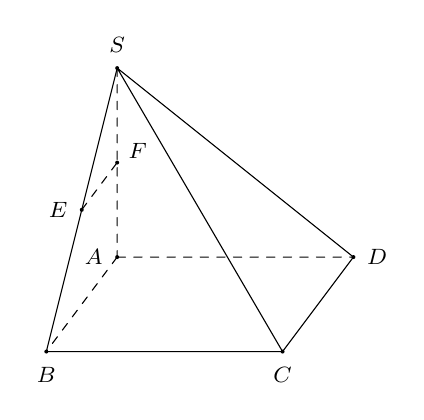
\begin{tikzpicture}[scale=0.6, font=\footnotesize, line join=round, line cap=round, >=stealth]
			\path (0,0)coordinate(A)
			--++(-1.5,-2) coordinate(B)
			--++(5,0) coordinate(C)
			(A)--+(5,0) coordinate (D)
			--+(0,4) coordinate (S);
			\draw (S)--(B)--(C)--(D)--cycle (S)--(C);
			\draw[dashed] (S)--(A) (A)--(B) (A)--(D);
			\foreach \p/\q in {A/180,B/-90,C/-90,D/0,S/90}{
				\path (\p) node[shift={(\q:3mm)}]{$\p$};
				\fill[black] (\p) circle (1.2pt);}
			\path (S)--(A) coordinate[pos=0.5] (F);
			\path (S)--(B) coordinate[pos=0.5] (E);
			\draw[dashed] (E)--(F);
			\path (F) node[shift={(30:3mm)}]{$F$};
			\path (E) node[shift={(180:3mm)}]{$E$};
			\fill[black] (F) circle (1.2pt);
			\fill[black] (E) circle (1.2pt);
		\end{tikzpicture}
	}
	\loigiai{
		\begin{itemize}
			\item Đường thẳng $SC$ và đường thẳng $EF$ chéo nhau.
			\item Ta có $EF$ là đường trung bình của tam giác $SAB$ nên $EF \parallel AB$. Mà $AB \parallel CD$ nên $EF \parallel CD$.
			\item Đường thẳng $AD$ và đường thẳng $SC$ chéo nhau.
			\item Đường thẳng $AE$ và đường thẳng $BF$ cắt nhau.
		\end{itemize}		
	}
\end{ex}

\begin{ex}%[1H4N1-2]%[KNTT - Lớp 11 - TRƯỜNG THPT NGUYỄN AN NINH - ĐỀ THI HK1]%[Quang Vinh NT] 
	Cho hình chóp $S.ABCD$. Khẳng định nào sau đây là \textbf{sai}?
	\choice
	{\True Đoạn thẳng $CD$ là một cạnh bên của hình chóp}
	{Điểm $S$ là đỉnh của hình chóp}
	{Tứ giác $ABCD$ là mặt đáy của hình chóp}
	{$\triangle SCD$ là một mặt bên của hình chóp}
	\loigiai{
		Đoạn thẳng $CD$ là cạnh đáy.
	}
\end{ex}

\begin{ex}%[1D2H1-3]%[Dự án đề kiểm tra toán khối 11 GHKI THPT NguyễnAnNinh]%[NGUYỄN HỮU ĐỨC]
%%%%%-----Câu 7.-----%%%%%
Cho dãy $(u_4)$, biết $u_n = \dfrac{2n^2 + 4}{n + 5}$. Tìm số hạng $u_4$?
	\choice
	{$u_4=6$}
	{$u_4=7$}
	{\True $u_4=4$}
	{$u_4=5$}
\loigiai{
	Thay $n=4$ vào dãy ta được $u_4 = \dfrac{2 \cdot 4^2 + 4}{4 + 5} = \dfrac{2 \cdot 16 + 4}{9} = \dfrac{32 + 4}{9} = \dfrac{36}{9} = 4$.
	}

\end{ex}
%%%%%-----Câu 8.-----%%%%%
\begin{ex}%[1H4H1-4]%[Dự án đề kiểm tra toán khối 11 GHKI THPT NguyễnAnNinh]%[NGUYỄN HỮU ĐỨC]
Cho tứ diện $ABCD$. Gọi $E$, $F$ là hai điểm lần lượt thuộc cạnh 
$BC$ và $CD$. Gọi $G$ là giao điểm của hai đường thẳng $EF$ và $BD$ (tham khảo hình vẽ). Khẳng định nào sau đây là \textbf{sai}?
	\choice
	{Đường thẳng $FG$ nằm trong mặt phẳng $(BCD)$}
	{Điểm $G$ thuộc mặt phẳng $(BCD)$}
	{\True Hai đường thẳng $AC$ và $BD$ cắt nhau}
	{Điểm $G$ là điểm chung của hai mặt phẳng $(ABD)$ và $(AEF)$}
\loigiai{
	\begin{center}
		\begin{tikzpicture}
			\def\a{4}
			\path (0:0) coordinate (B)
			++(0:\a) coordinate (D)
			($(B)+(-70:\a/2)$) coordinate (C)
			($(B)+(75:.85*\a)$) coordinate (A)
			($(C)!.5!(B)$) coordinate (E)
			($(C)!.7!(D)$) coordinate (F)
			(intersection of E--F and B--D) coordinate (G);
			\draw[dashed] (B)--(D) (E)--(F);
			\draw (A)--(B)--(C)--(D) (C)--(A) (A)--(D) (F)--(G) (G)--(D);
			\foreach \x/\g in {F/-90,B/180,C/-90,D/60,A/90,E/180,G/60}
			\fill (\x) circle (1pt)
			($(\g:3mm)+(\x)$) node {$\x$}; 
		\end{tikzpicture}
		
\end{center}
	Hai đường thẳng $AC$ và $BD$ chéo nhau.
}
\end{ex}
%%%%%-----Câu 9.-----%%%%%
\begin{ex}%[1D1N4-7]%[Dự án đề kiểm tra toán khối 11 GHKI THPT NguyễnAnNinh]%[NGUYỄN HỮU ĐỨC]
Hình vẽ bên là đồ thị hàm số nào dưới đây
\begin{center}
	\begin{tikzpicture}[>=stealth,scale=0.77,transform shape] 
		\path
		({-2.5*pi},0) coordinate (X1)
		({-2*pi},0) coordinate (X2)
		({-1.5*pi},0) coordinate (X3)
		({-pi},0) coordinate (X4)
		({-0.5*pi},0) coordinate (X5)
		(0,0) coordinate (O)
		({0.5*pi},0) coordinate (X6)
		({pi},0) coordinate (X7)
		({1.5*pi},0) coordinate (X8)
		({2*pi},0) coordinate (X9)
		({2.5*pi},0) coordinate (X10)
		({-pi},-2) coordinate (A)
		({pi},-2) coordinate (B)
		;
		\draw[->] (-9.5,0) -- (9.5,0) node[below] {\small $x$};
		\draw[->] (0,-1.5) -- (0,1.8) node[right] {\small $y$};
		\draw [dotted] (X2)--({-2*pi},1)--({2*pi},1)--({2*pi},0) (X4)--({-pi},-1)--({pi},-1)--({pi},0) 
		({-pi},0) -- (A) ({pi},0) -- (B);
		\foreach \x/\g/\z in {X1/125/-\tfrac{5\pi}{2},X2/-90/-2\pi,X3/-120/-\tfrac{3\pi}{2},X4/90/-\pi,X5/110/-\tfrac{\pi}{2},X6/-120/\tfrac{\pi}{2},X7/90/\pi,X8/120/\tfrac{3\pi}{2},X9/-90/2\pi,X10/-120/\tfrac{5\pi}{2}} 
		\fill[black] (\x) circle(1pt) +(\g:5mm) node {$\z$};
		\draw [<->] ({-pi},-1.7)--({pi},-1.7) ; 
		\draw (0,0) node[below right]{$O$} (0,-1.7) node[below]{$T=2\pi$}
		(0,1) node[above right]{$1$} (0,-1) node[below right]{$-1$}
		;
		\clip (-9.5,-1.4) rectangle (9.5,1.6) ;
		\draw[thick,samples=100,domain=-9.3:9.3] plot(\x,{cos((\x)*180/pi)});
		
	\end{tikzpicture}
\end{center}
\choice
{$y=\cot x$}
{\True $y=\cos x$}
{$y=\sin x$}
{$y=\tan x$}
\loigiai{
	Hàm số đồng biến trên mỗi khoảng $(-\pi+k 2 \pi ; k 2 \pi)$ và nghịch biến trên mỗi khoảng $\break(k 2 \pi ; \pi+k 2 \pi), k \in \mathbb{Z}$;
	Có đồ thị là một đường hình sin đối xứng qua trục tung $\Rightarrow y=\cos x$.
}
\end{ex}%%%%%-----Câu 10.-----%%%%%
\begin{ex}%[1H4H3-2]%[Dự án đề kiểm tra toán khối 11 GHKI THPT NguyễnAnNinh]%[NGUYỄN HỮU ĐỨC]
Cho hình chóp $S.ABCD$ có đáy $ABCD$ là hình bình hành tâm $O$. Gọi $E$, $F$ lần lượt là trung điểm của cạnh $SB$ và $SA$ (xem hình). Chọn khẳng định đúng.
\choice
{Đường thẳng $OE$ song song với mặt phẳng $(SBD)$}
{\True Đường thẳng $CD$ song song với mặt phẳng $(OEF)$}
{Đường thẳng $OF$ song song với mặt phẳng $(SAC)$}
{Đường thẳng $EF$ song song với mặt phẳng $(SAB)$}
\begin{center}
	\begin{tikzpicture}
		\def\a{3}
		\path (0:0) coordinate (A)
		++(0:\a) coordinate (D)
		++(-135:.6*\a) coordinate (C)
		($(A)+(C)-(D)$) coordinate (B)
		($(A)+(94:\a)$) coordinate (S)
		(intersection of A--C and B--D) coordinate (O)
		($(S)!.5!(B)$) coordinate (E)
		($(A)!.5!(S)$) coordinate (F);
		\draw[dashed] (B)--(A)--(D) (A)--(S) (B)--(D) (C)--(A) (E)--(F) (O)--(F) (O)--(E);
		\draw (B)-- (C)--(D) (B)--(S) (C)--(S) (D)--(S);
		\foreach \x/\g in {A/145,B/-135,C/-45,D/45,S/90,E/-150,F/5,O/45}
		\fill (\x) circle (1pt)
		($(\g:3mm)+(\x)$) node {$\x$}; 
	\end{tikzpicture}
\end{center}
\loigiai{
	Do $E$, $F$ lần lượt là trung điểm của cạnh $SB$ và $SA$ nên $AB$ song song $EF$.\\
	Mà $AB$ song song $CD$ nên $CD$ song song với mặt phẳng $(OEF)$.
	
}
\end{ex}%%%%%-----Câu 11.-----%%%%%
\begin{ex}%[1H4H3-2]%[Dự án đề kiểm tra toán khối 11 GHKI THPT NguyễnAnNinh]%[NGUYỄN HỮU ĐỨC]
Cho hình chóp $S.ABCD$ có đáy $ABCD$ là hình bình hành. Khẳng định nào sau đây là \textbf{sai}?
\choice
{$AD \parallel (SBC)$}
{$AB \parallel (SCD)$}
{\True $AC \parallel (SCD)$}
{$CD \parallel (SAB)$}
\loigiai{
	\begin{center}
		\begin{tikzpicture}
			\def\a{3}
			\path (0:0) coordinate (A)
			++(0:\a) coordinate (D)
			++(-135:.6*\a) coordinate (C)
			($(A)+(C)-(D)$) coordinate (B)
			($(A)+(94:\a)$) coordinate (S)
			(intersection of A--C and B--D) coordinate (O)
			($(S)!.5!(B)$) coordinate (E)
			($(A)!.5!(S)$) coordinate (F);
			\draw[dashed] (B)--(A)--(D) (A)--(S) (B)--(D) (C)--(A);
			\draw (B)-- (C)--(D) (B)--(S) (C)--(S) (D)--(S);
			\foreach \x/\g in {A/145,B/-135,C/-45,D/45,S/90,O/45}
			\fill (\x) circle (1pt)
			($(\g:3mm)+(\x)$) node {$\x$}; 
		\end{tikzpicture}
	\end{center}
	Do $AC$ cắt $(SCD)$ tại $C$.
}
\end{ex}
\begin{ex}%[1D1H5-5]%[Dự án đề kiểm tra toán khối 11 GHKI THPT NguyễnAnNinh]%[NGUYỄN HỮU ĐỨC]
	Tất cả các nghiệm của phương trình $\sin 2x = \sin x$ là
	\choice
	{$x = k2\pi; x = \dfrac{\pi}{3} + k2\pi, (k \in \mathbb{Z})$}
	{\True $x = k2\pi; x = \dfrac{\pi}{3} + k\dfrac{2\pi}{3}, (k \in \mathbb{Z})$}
	{$x = k2\pi; x = k\dfrac{2\pi}{3}, (k \in \mathbb{Z})$}
	{$x = k2\pi; x = \dfrac{\pi}{3} + k\pi, (k \in \mathbb{Z})$}
	\loigiai{Ta có
		$\begin{aligned}[t]
			%& \sin 2x = \sin x\\ 
			&  \sin 2x=\sin x\\
			& \Leftrightarrow \hoac{&x=k2\pi \\ 
			&x=\dfrac{\pi}{3}+k\dfrac{2\pi}{3}}, (k\in \mathbb{Z}).
		\end{aligned}$
	}
\end{ex}

\Closesolutionfile{ans}

%\indapan{6}{ans-ABCD}

%\cauds

\begin{center}
	\textbf{PHẦN 2 - Câu trắc nghiệm đúng sai. Trong mỗi ý a,b,c,d ở mỗi câu, thí sinh chọn đúng hoặc sai}
\end{center}
\setcounter{ex}{0}
\Opensolutionfile{ans}[ans-DS]
%%%=============EX_1=============%%%
\begin{ex}%[1D1H3-3]%[Dự án đề kiểm tra Toán 11 GHKI NH24-25- Nguyễn Trần Anh Tuấn]%[THPT Nguyễn An Ninh]
	Cho $\sin \alpha=\dfrac{7}{25}$ và $\left(\dfrac{\pi}{2} < \alpha < \pi\right)$; $\cos \beta=-\dfrac{5}{13}$ và  $\left(\pi < \beta < \dfrac{3\pi}{2}\right)$.
	\choiceTF
	{$\cos (\alpha+\beta)=\cos \alpha \cdot \cos \beta+\sin \alpha \cdot \sin \beta$}
	{$\cos \alpha=\sqrt{1+\sin ^2\alpha}$}
	{$\cos (\alpha+\beta)=\dfrac{36}{325}$}
	{$\cos 4\beta=-\dfrac{239}{2861}$}
	\loigiai{
		\begin{itemchoice}
			\itemch \textbf{Sai}.\\
			$\cos (\alpha+\beta)=\cos \alpha \cdot \cos \beta-\sin \alpha \cdot \sin \beta$
			\itemch \textbf{Sai}.\\
			Với $\alpha \in\left(\dfrac{\pi}{2} ; \pi\right)$ thì $\cos \alpha<0$.\\
			Ta có 
			$\begin{aligned}[t]
				\sin^2 \alpha+\cos^2 \alpha&=1\\
				%\cos ^2 \alpha &=1-\sin ^2 \alpha \\
				\Rightarrow \cos \alpha &=-\sqrt{1-\sin ^2 \alpha}
			\end{aligned}$
			\itemch \textbf{Sai}.\\
			Ta có 
			$\begin{aligned}[t]
				\cos \alpha &=-\sqrt{1-\sin ^2 \alpha}\\
				&=-\sqrt{1-\left(\dfrac{7}{25}\right)^2}\\
				&=-\dfrac{24}{25}.
			\end{aligned}$\\
			Tương tự với $\beta \in\left(\pi < \beta < \dfrac{3\pi}{2}\right)$ thì $\sin \beta<0$.\\
			Ta có 
			$\begin{aligned}[t]
				\sin \beta &=-\sqrt{1-\cos ^2 \beta}\\
				&=-\sqrt{1-\left(-\dfrac{5}{13}\right)^2}\\
				&=-\dfrac{12}{13}.
			\end{aligned}$\\
			$\begin{aligned}[t]
				\cos (\alpha+\beta)&=\cos \alpha \cdot \cos \beta-\sin \alpha \cdot \sin \beta\\
				&=-\dfrac{24}{25} \cdot\left(-\dfrac{5}{13}\right)-\dfrac{7}{25} \cdot\left(-\dfrac{12}{13}\right)\\
				&=\dfrac{204}{325}.
			\end{aligned}$
			\itemch \textbf{Sai}.\\
			Ta có 
			$\begin{aligned}[t]
				\cos 4 \beta & =1-2 \sin^2 2 \beta \\
				& =1-2\left(2 \cdot \sin \beta \cdot \cos \beta\right)^2 \\
				& =1-2 \cdot\left[2 \cdot\left(-\dfrac{12}{13}\right) \cdot\left(\dfrac{-5}{13}\right)\right]^2 \\
				& =-\dfrac{239}{28561}.
			\end{aligned}$
		\end{itemchoice}
	}
\end{ex}
%%%=============EX_2=============%%%
\begin{ex}%[1H4H3-2]%[Dự án đề kiểm tra Toán 11 GHKI NH24-25- Nguyễn Trần Anh Tuấn]%[THPT Nguyễn An Ninh]
	Cho hình chóp $S.ABCD$ có đáy là hình thang với $AD$ là đáy lớn, $O$ là giao điểm của $AC$ và $BD$. Gọi $M$, $N$, $P$ lần lượt là trung điểm của $SA$, $SD$, $SB$. Xét tính đúng, sai của các mệnh đề sau:
	\choiceTF
	{Đường thẳng $BD$ cắt $SC$ tại một điểm}
	{\True Giao tuyến của hai mặt phẳng $(SAC)$ và $(SBD)$ là đường thẳng $SO$}
	{\True Đường thẳng $MN$ song song với đường thẳng $BC$}
	{\True Đường thẳng $BD$ song song với mặt phẳng ($MNP$)}
	\loigiai{
		\begin{center}
			\begin{tikzpicture}[line join = round, line cap = round,>=stealth,thick,font=\footnotesize,scale=1]
				\path (0,0) coordinate(A)
				(6,0)  coordinate(D)
				(-60:3) coordinate (B)
				(B)+(0:2) coordinate (C)
				
				(intersection of A--C and B--D) coordinate (O)
				(O)+(90:6)  coordinate (S)
				($(S)!0.5!(A)$) coordinate (M)
				($(S)!0.5!(B)$) coordinate (P)
				($(S)!0.5!(D)$) coordinate (N)
				;
				\draw (A)--(B)--(C)--(D)
				\foreach \x in {A,B,C,D}{(S)--(\x)}
				(M)--(P)node[white]{·–·};
				\draw[dashed] (A)--(C) (B)--(D) (S)--(O) (A)--(D) (M)--(N) (P)--(N);
				\foreach \i/\g in {A/135,B/-135,C/-45,D/45,S/90,M/135,P/-135,N/45,O/-90}{
					\draw[fill=black](\i) circle (1.5pt) ($(\i)+(\g:3mm)$) node[scale=1]{$\i$};}
			\end{tikzpicture}
		\end{center}
		\begin{itemchoice}
			\itemch \textbf{Sai}.\\
			$BD$, $SC$ chéo nhau.
			\itemch \textbf{Đúng}.\\
			Trong mp (ABCD) ta có $ O=AC\cap BD$.\\
			$\Rightarrow O \in(SAC) \cap(SBD)$.\\
			Mặt khác: $S \in(SAC) \cap(SBD)$.\\
			Vậy $(SAC) \cap(SBD)=SO$.
			\itemch \textbf{Đúng}.\\
			Xét $\triangle SAD$ ta có\\
			$M$ là trung điểm của  $SA$,\\
			$N$ là trung điểm của  $SD$,\\
			Suy ra $MN$ là đường trung bình $\triangle SAD$.\\
			$\Rightarrow MN \parallel AD$.\\
			Mà $AD \parallel BC$.\\
			Vậy $MN \parallel BC$.
			\itemch \textbf{Đúng}.
			Xét $\triangle SBD$ ta có\\
			$N$ là trung điểm của  $SD$,\\
			$B$ là trung điểm của  $SB$,\\
			Suy ra $NP$ là đường trung bình $\triangle SBD$.\\
			$\Rightarrow NP \parallel BD$.\\
			Mà $NP \subset (MNP)$ và $BD \not\subset (MNP)$.\\
			Vậy $BD \parallel (MNP)$.
		\end{itemchoice}
		
	}
\end{ex}
%%%=============EX_3=============%%%
\begin{ex}%[1D2H2-6]%[Dự án đề kiểm tra Toán 11 GHKI NH24-25- Nguyễn Trần Anh Tuấn]%[THPT Nguyễn An Ninh]
	Cho dãy số $(u_n)$ với $u_n=21-6n$.
	\choiceTF
	{Số hạng thứ $2\,025$ của dãy $(u_n)$ bằng $12\,129$}
	{\True Với mọi số nguyên dương $n$, ta có dãy số $(u_n)$ giảm}
	{Dãy số $(u_n)$ là dãy cấp số cộng có số hạng đầu bằng $-6$ và có công sai bằng $15$}
	{\True Tổng của $3\,024$ số hạng đầu tiên của dãy số $(u_n)$ bằng $-27\,379\,296$}
	\loigiai{
		\begin{itemchoice}
			\itemch \textbf{Sai}.\\
			$u_{2\,025}=21-6\cdot 2\,025=-12\,129$.
			\itemch \textbf{Đúng}.\\
			Với mọi số nguyên dương $n$ ta xét\\
			$u_n=21-6n$, $u_{n+1}=21-6(n+1)$.\\
			Ta có $u_{n+1}-u_n=-6$.\\
			Suy ra $u_n$ là dãy giảm.
			\itemch \textbf{Sai}.\\
			Ta có $u_{n+1}-u_n=-6$ suy ra $(u_n)$ là cấp số cộng với $\heva{& u_1=15 \\ & d=-6.}$
			\itemch \textbf{Đúng}.\\
			$S_{3\,024}=3\,024 \cdot(15)+\dfrac{3\,024 \cdot 3\,023 \cdot(-6)}{2}=-27\,379\,296$.
		\end{itemchoice}
	}
\end{ex}
%%%=============EX_4=============%%%
\begin{ex}%[1D1H5-5]%[Dự án đề kiểm tra Toán 11 GHKI NH24-25- Nguyễn Trần Anh Tuấn]%[THPT Nguyễn An Ninh]
	Cho phương trình lượng giác $\sin x=\dfrac{1}{2} \qquad(1)$
	\choiceTF
	{\True Phương trình $\sin x=\dfrac{1}{2} \Leftrightarrow \sin x=\sin \dfrac{\pi}{6}$}
	{Phương trình (1) có các nghiệm là $x=\dfrac{\pi}{6}+k 2\pi$ và $x=-\dfrac{\pi}{6}+k 2\pi$, $(k \in \mathbb{Z})$}
	{Phương trình (1) có nghiệm âm lớn nhất là $-\dfrac{\pi}{6}$}
	{\True Phương trình có nghiệm dương nhỏ nhất bằng $\dfrac{\pi}{6}$}
	\loigiai{
		\begin{itemchoice}
			\itemch \textbf{Đúng}.\\
			$\sin \dfrac{\pi}{6}=\dfrac{1}{2}$.
			\itemch \textbf{Sai}.\\
			$\begin{aligned}[t]
				& \sin x=\dfrac{1}{2} \\ 
				& \Leftrightarrow \sin x=\sin \dfrac{\pi}{6} \\
				& \Leftrightarrow \hoac{&x=\dfrac{\pi}{6}+k2\pi \\ &x=\dfrac{5\pi}{6}+K2\pi}, (k\in \mathbb{Z})
			\end{aligned}$
			\itemch \textbf{Sai}.\\
			Với $x=\dfrac{\pi}{6}+k2\pi$ thì
			\begin{eqnarray*} 
				\dfrac{\pi}{6}+k2\pi & <&0 \\ 
				k & <&-\dfrac{1}{12}
			\end{eqnarray*}
			Chọn $k=-1$ ta có $x=-\dfrac{11\pi}{6}$.\\
			Với $x=\dfrac{5\pi}{6}+K2\pi$ thì
			\begin{eqnarray*} 
				\dfrac{5\pi}{6}+k2\pi & <&0 \\ 
				k & <&-\dfrac{5}{12}
			\end{eqnarray*}
			Chọn $k=-1$ ta có $x=-\dfrac{7\pi}{6}$.\\
			Vậy nghiệm âm lớn nhất là $x=-\dfrac{7\pi}{6}$.
			\itemch \textbf{Đúng}.\\
			Với $x=\dfrac{\pi}{6}+k2\pi$ thì
			\begin{eqnarray*} 
				\dfrac{\pi}{6}+k2\pi & >&0 \\ 
				k & >&-\dfrac{1}{12}
			\end{eqnarray*}
			Chọn $k=0$ ta có $x=\dfrac{\pi}{6}$.\\
			Với $x=\dfrac{5\pi}{6}+k2\pi$ thì
			\begin{eqnarray*} 
				\dfrac{5\pi}{6}+k2\pi & >&0 \\ 
				k &>&-\dfrac{5}{12}
			\end{eqnarray*}
			Chọn $k=0$ ta có $x=\dfrac{5\pi}{6}$.\\
			Vậy nghiệm dương nhỏ nhất là $x=\dfrac{\pi}{6}$.
		\end{itemchoice}
	}
\end{ex}
\Closesolutionfile{ans}

\begin{center}
	\textbf{PHẦN 3 - Câu trắc nghiệm trả lời ngắn}
\end{center}
\setcounter{ex}{0}

\Opensolutionfile{ans}[ans-KQ]
%Câu TL ngắn 1 (Sửa format shortans)
\begin{ex}%[1D1H4-8]%[Dự án đề kiểm tra Toán 11 GHKI NH24-25- Nguyễn Hữu Đức]%[THPT-NguyenAnNinh - Tp HCM]
	Độ sâu $D(t)$ mét của nước ở một cảng biển sau $t$ giờ kể từ lúc nửa đêm được tính bởi công thức $D(t) = 4 \cos \left( \frac{\pi t}{6} \right) + 6$; $(0\le t\le 24)$. Độ sâu của nước ở cảng này sau $14$ giờ là bao nhiêu mét?
	\shortans[oly]{8}
	\loigiai{
		Thay $t = 14$ vào công thức $D(t)$:
		\[
		D(14) = 4 \cos \left( \frac{\pi \cdot 14}{6} \right) + 6 = 4 \cos \left( \frac{7\pi}{3} \right) + 6 = 4 \cdot \dfrac{1}{2} + 6 = 8.
		\]
		Vậy độ sâu của nước là $8$ mét.
	}
\end{ex}

%Câu TL ngắn 2 (Sửa format shortans)
\begin{ex}%[1H4H1-4]%[Dự án đề kiểm tra Toán 11 GHKI NH24-25- Nguyễn Hữu Đức]%[THPT-NguyenAnNinh - Tp HCM]
	Trong hình chóp $S.ABCD$ có đáy $ABCD$ là hình thang, $AD$ là đáy lớn. Gọi $E$ là trung điểm của cạnh $SA$. Đường thẳng $SD$ cắt mặt phẳng $(EBC)$ tại $F$. Đường thẳng $AF$ cắt $DE$ tại $K$. Tính tỉ số $\dfrac{KD}{KE}$.
	\shortans[oly]{2}
	\loigiai{
		\begin{center}
			\begin{tikzpicture}[scale=0.8]
				\def\a{4}
				\path (0:0) coordinate (A)
				++(0:\a) coordinate (D)
				($(A)+(-70:\a/2)$) coordinate (B)
				($(B)+(D)-(A)$) coordinate (Ct)
				($(B)!.5!(Ct)$) coordinate (C)
				($(A)+(75:.85*\a)$) coordinate (S)
				($(A)!.5!(S)$) coordinate (E)
				($(D)!.5!(S)$) coordinate (F)
				(intersection of A--F and E--D) coordinate (K);
				\draw[dashed] (A)--(D) (E)--(C) (E)--(F) (E)--(D) (A)--(F);
				\draw (A)--(B)--(C)--(D) (A)--(S) (E)--(B)
				(B)--(S) (C)--(S) (D)--(S);
				\draw[dashed] (E)--(F)node[above]{$d$};
				\foreach \x/\g in {A/180,E/180,B/-135,C/-45,D/0,F/10,S/90,K/10}
				\fill (\x) circle (1pt)
				($(\g:3mm)+(\x)$) node {$\x$};
			\end{tikzpicture}
		\end{center}
		Giao tuyến của $(EBC)$ và $(SAD)$ là đường thẳng $EF \parallel BC \parallel AD$. Vì $E$ là trung điểm $SA$ nên $F$ là trung điểm $SD$.\\
		Xét $\triangle SAD$, $DE$ và $AF$ là hai đường trung tuyến cắt nhau tại $K$, suy ra $K$ là trọng tâm.\\
		Do đó $\dfrac{KD}{KE}=2$.
	}
\end{ex}

%Câu TL ngắn 3 (Sửa đáp án và lời giải)
\begin{ex}%[1D1V2-5]%[Dự án đề kiểm tra Toán 11 GHKI NH24-25- Nguyễn Hữu Đức]%[THPT-NguyenAnNinh - Tp HCM]
	Một xe đạp đang di chuyển, van $M$ của bánh xe quay quanh trục $O$ theo chiều kim đồng hồ với tốc độ góc không đổi $10$ rad/s. Khoảng cách từ van $M$ đến mặt đất là đoạn $MH$. Ban đầu, van $M$ nằm ở vị trí $A$ (xem hình). Hỏi sau 2 phút khoảng cách từ van $M$ đến mặt đất là bao nhiêu cm? Biết bán kính bánh xe $R = 35$ cm. Giả sử độ dày của lốp xe không đáng kể. Làm tròn kết quả đến hàng phần mười.
	
	\shortans[oly]{38,1}
	\loigiai{
		\begin{center}
			\begin{tikzpicture}[scale=0.8]
					\draw[thick] (-4,-2) -- (4,-2) node[anchor=north] {Mặt đất};
					\draw[->] (-3,0) -- (3,0) node[anchor=north west] {$x$};
					\draw[->] (0,-2) -- (0,3) node[anchor=east] {$y$};
					\draw[thick] (0,0) circle (2);
					\draw[thick] (1.3,1.5) -- (1.3,-2) node[below] {H};
					\draw[thick] (0,0) -- (2,0) node[anchor=north west] {A};
					\draw[thick] (0,0) -- (1.3,1.5) node[above right] {M};
					\node at (0,0) [below left] {O};
			\end{tikzpicture}
		\end{center}
		Đổi $t = 2 \text{ phút} = 120 \text{ giây}$.\\
		Góc quay được: $\theta = -10 \cdot 120 = -1\,200 \text{ rad}$ (dấu âm do quay cùng chiều kim đồng hồ).\\
		Độ cao của tâm $O$ so với mặt đất là $R = 35$ cm.\\
		Vị trí độ cao của $M$ so với tâm $O$ là $y_M = R \sin(-1\,200)$.\\
		Khoảng cách từ $M$ đến mặt đất:
		\[ h = R + y_M = 35 + 35\sin(-1\,200) \approx 35 + 35(0{,}088) \approx 38{,}1 \text{ cm}. \]
	}
\end{ex}

%Câu TL ngắn 4 (Sửa format shortans)
\begin{ex}%[1D2V2-7]%[Dự án đề kiểm tra Toán 11 GHKI NH24-25- Nguyễn Hữu Đức]%[THPT-NguyenAnNinh - Tp HCM]
	Khán đài A của một sân vận động có $3\,456$ chỗ ngồi, hàng ghế đầu tiên có $15$ chỗ ngồi và mỗi hàng ghế sau có thêm $6$ chỗ so với hàng ghế ngay trước nó. Hỏi khán đài A của sân vận động có bao nhiêu hàng ghế?
	\shortans[oly]{32}
	\loigiai{
		Dãy số ghế là cấp số cộng với $u_1 = 15, d = 6, S_n = 3\,456$.\\
		Ta có phương trình:
		\[ 3\,456 = \dfrac{n}{2} [2\cdot 15 + (n-1)6] \Leftrightarrow 3n^2 + 12n - 3\,456 = 0 \]
		Giải phương trình được $n=32$ (nhận) hoặc $n=-36$ (loại).\\
		Vậy có $32$ hàng ghế.
	}
\end{ex}

%-----Câu 5
\begin{ex}%[1H4H3-3]%[Dự án đề kiểm tra Toán 11 GHKI NH24-25- Nguyễn Hữu Đức]%[THPT-NguyenAnNinh - Tp HCM]
	Cho hình chóp $S.ABCD$ có đáy $ABCD$ là hình bình hành. Mặt phẳng $(\alpha)$ qua $BD$ và song song với $SA$, mặt phẳng $(\alpha)$ cắt $SC$ tại $K$. Tính tỉ số $\dfrac{SK}{SC}$.
	\shortans[oly]{0,5}
	\loigiai{
	\immini{
		Gọi $O=AC\cap BD$. Giao tuyến của $(\alpha)$ và $(SAC)$ đi qua $O$ và song song với $SA$ (do $SA \parallel (\alpha)$).\\
		Trong $\triangle SAC$, đường thẳng qua trung điểm $O$ của $AC$ và song song với $SA$ sẽ cắt $SC$ tại trung điểm $K$.\\
		Vậy $\dfrac{SK}{SC} = 0{,}5.}{
			\begin{tikzpicture}[font=\footnotesize, line join=round, line cap=round, >=stealth,scale=0.8]
				\path
				(0,0) coordinate (A) 
				(-2,-2) coordinate (B)
				(3,-2) coordinate (C)
				(5,0) coordinate (D)
				(0.5,4) coordinate (S)
				($(A)!.5!(C)$) coordinate (O)
				($(S)!.5!(C)$) coordinate (K)
				%(intersection of M--N and A--C) coordinate (I)
				%(intersection of S--O and B--P) coordinate (H)
				;
				\draw 
				(S)--(B)--(C)--(D)--cycle
				(S)--(C) (B)--(K)--(D);
				\draw [dashed] (S)--(A)--(D)--(B)--(A)--(C) (K)--(O);
				%			\draw (-2,1.5)--(2,5.5)node[above]{$d$};
				\foreach \x/\g in
				{A/150,B/180,C/0,D/0,S/90,O/-90,K/40}
				\fill (\x) circle (1pt)
				($(\x)+(\g:3mm)$) node{$\x$};
			\end{tikzpicture} }
	}
\end{ex}

%-----Câu 6
\begin{ex}%[1H4H3-3]%[Dự án đề kiểm tra Toán 11 GHKI NH24-25- Nguyễn Hữu Đức]%[THPT-NguyenAnNinh - Tp HCM]
	\immini{Từ một vị trí $A$, người ta buộc hai sợi cáp $AB$ và $AD$ đến một cái trụ cao $CB = 16$ m được dựng vuông góc với mặt đất, chân trụ ở vị trí $C$. Biết $CD = 10$ m và $AC = 11$ m (xem hình). Tính số đo (theo độ) góc nhọn $\widehat {BAD}$ tạo bởi hai sợi dây cáp đó. Kết quả làm tròn đến độ.}{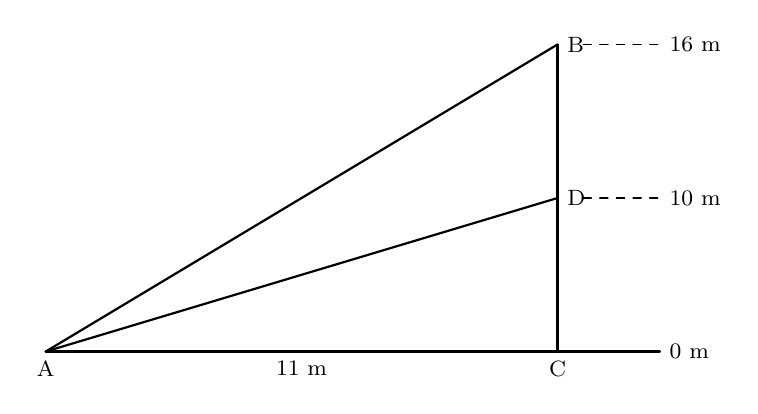
\begin{tikzpicture}[font=\footnotesize, line join=round, line cap=round, >=stealth,scale=0.65]
					\draw[thick] (0,0) -- (12,0);
					\draw[thick] (10,0) -- (10,6);
					\node at (0,0) [below] {A};
					\node at (10,6) [right] {B};
					\node at (10,0) [below] {C};
					\node at (10,3) [right] {D};
					\draw[thick] (0,0) -- (10,6);
					\draw[thick] (0,0) -- (10,3);
					\node at (5,0) [below] {11 m};
					\draw[dashed] (10.5,6) -- (12,6);
					\draw[dashed] (10.5,3) -- (12,3);
					\draw[dashed] (10,0) -- (12,0);
					\node at (12,6) [right] {$16$ m};
					\node at (12,3) [right] {$10$ m};
					\node at (12,0) [right] {$0$ m};
				\end{tikzpicture}}
	\shortans[oly]{13}
	\loigiai{
		Ta có $\tan \widehat{CAD}=\dfrac{10}{11}$, $\tan \widehat{CAB}=\dfrac{16}{11}$.\\
		$\tan \widehat{DAB}=\tan \left(\widehat{CAB}-\widehat{CAD}\right)=\dfrac{\frac{16}{11}-\frac{10}{11}}{1+\frac{16}{11}\cdot \frac{10}{11}}=\dfrac{66}{281}$.\\
		$\Rightarrow \widehat{DAB} \approx 13^{\circ}$}
\end{ex}

\Closesolutionfile{ans}



